\chapter{Аналитический раздел}
Гидро- и аэродинамика макроскопически описывается уравнениями Навье--Стокса. Они связывают давление, плотность и скорость жидкости в каждой точке пространства в каждый момент времени~--- в зависимости от начальных и граничных условий и параметров среды.

В случае вязкой слабосжимаемой жидкости система состоит из двух уравнений:

\begin{enumerate}
  \item уравнения движения
    \begin{equation} \label{eq:momentum}
      \rho\left(\frac{\partial}{\partial t}+\vect u\cdot\nabla\right)\vect u=-\nabla p+\mu\laplace\vect u+\vect f
    \end{equation}
  \item уравнения неразрывности
    \begin{equation} \label{eq:continuity}
      \nabla\cdot\vect u=0,
    \end{equation}
\end{enumerate}
\begin{conditions}
  $\nabla$ & оператор набла;\\
  $\laplace$ & векторный лапласиан;\\
  $\rho$ & плотность $\left[\frac{\text{кг}}{\text{м}^3}\right]$;\\
  $t$ & время, с;\\
  $\vect u$ & векторное поле скоростей, $\left[\frac{\text{м}}{\text{c}}\right]$;\\
  $p$ & давление, Па;\\
  $\mu$ & коэффициент динамической вязкости, $\left[\frac{\text{Н}\cdot\text{с}}{\text{м}^2}\right]$;\\
  $\vect f$ & векторное поле внешних объёмных сил, $\left[\frac{\text{Н}}{\text{м}^3}\right]$.
\end{conditions}

Однако в аналитическом виде решения этих уравнений найдены лишь в некоторых частных случаях, в общем же случае показана невозможность решения данной <<проблемы тысячелетия>> существующими на настоящий момент средствами \cite{terence}. Поэтому нет полного понимания свойств уравнений Навье--Стокса, а значит численное моделирование остаётся основным способом исследования поведения жидкости.

Существует три фундаментальных подхода к данной задаче: сеточный метод, так называемый метод Эйлера, метод решёточных уравнений Больцмана и метод гидродинамики сглаженных частиц, известный как метод Лагранжа.


\section{Метод решёточных уравнений Больцмана}
Метод основан на дискретизации кинетического уравнения Больцмана, которое описывает, как меняется плотность распределения частиц по скоростям в каждой точке пространства со временем. Если проинтегрировать распределение частиц по скоростям в данной точке, то можно получить макроскопическую скорость для этой точки. Другими словами, макроскопически уравнение Больцмана эквивалентно уравнению Навье-Стокса.

Несмотря на то, что для плотных жидкостей уравнение Больцмана в общем виде не применимо, оно показывает неплохие результаты. В методе используется замена нижележащего уровня абстракций (микроскопическое уравнение для плотных жидкостей) физически неправильной реализацией (микроскопическое уравнение для разреженных газов), но так, что верхний уровень (макроскопическое уравнение Навье-Стокса) описывается верно.

Уравнение Больцмана, используемое в данном методе:
\begin{equation}
  f\left(\vect r+\vect vdt, \vect v+\frac{\vect F}{m}dt, t+dt\right)-f(\vect r, \vect v, t)=-\frac{f-f_0}{\tau}dt
\end{equation}
\begin{conditions}
  $f$ & функция распределения плотности вероятности частиц;\\
  $\vect r$ & положение молекулы;\\
  $\vect v$ & скорость молекулы;\\
  $t$ & время;\\
  $\vect F$ & внешняя сила;\\
  $m$ & масса молекулы;\\
  $f_0$ & равновесная функция распределения;\\
  $\tau$ & время релаксации.
\end{conditions}

Чтоб получить возможность моделировать динамику непрерывного уравнения Больцмана на компьютере, необходимо его дискретизировать. Для этого вводится равномерная сетка пространственных координат с одинаковым шагом сетки по всем осям. Поведение жидкости определяется именно в узлах сетки. Фактически, разрешается молекулам находиться только в определенных пространственных узлах. Кроме того, нужно дискретизировать время, так как необходимо определять состояние жидкости в равноотстоящие друг от друга моменты времени. Кроме того, молекулам позволяется иметь только определенные значения скорости~--- такие, что за шаг по времени они успевают перейти в какой-нибудь соседний узел. Эти разрешенные направления будут одинаковыми для всех пространственных узлов. Очевидно, что по диагональным направлениям скорости частиц будут больше, чем по недиагональным.

Интуитивно можно заключить, что при бесконечно малом шаге времени и шаге пространственной решетки эта дискретная система переходит в обычное уравнение Больцмана, которое, в свою очередь, переходит к уравнению Навье--Стокса в макроскопическом пределе.

\begin{figure}[h]
  \centering
  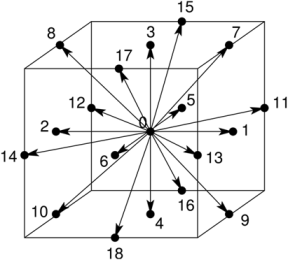
\includegraphics[width=.45\textwidth]{boltzmann.png}
  \caption{Возможные направления движения частицы.}
\end{figure}

Таким образом, на каждом шаге вычислительной схемы необходимо <<распространить>> частицы, то есть переместить частицы, летевшие из одного узла в соседний (проделать это для всех частиц и направлений). После этого необходимо пересчитать массы, скорости, равновесные функции распределения. Наконец, необходимо <<столкнуть>> частицы, прилетевшие в данный узел, то есть перераспределить частицы по направлениям.

Преимущества метода:
\begin{itemize}
  \item гибкость при задании граничных условий, поскольку такие условия задаются на макроскопическом уровне, а сам метод формулируется на микроскопическом уровне (потоки молекул);
  \item возможность моделировать поток смеси жидкостей или газов с разными параметрами;
  \item лёгкость распараллеливания.
\end{itemize}

Недостатки метода:
\begin{itemize}
  \item сложность задания начальных условий: в начале моделирования необходимо задать потоки молекул из каждого узла по всем разрешенным направлениям;
  \item использование ограничено малыми скоростями;
  \item обладает неустойчивым поведением на границе подвижных тел.
\end{itemize}


\section{Сеточный метод Эйлера}
Для моделирования поведения жидкости необходимо иметь состояние в любой момент времени. Наиболее важной характеристикой для представления является скорость, потому что скорость определяет, как жидкость движется. Скорость изменяется во времени и пространстве, поэтому представляется в виде векторного поля, которое накладывается на дискретную сетку.

\begin{figure}[h]
  \centering
  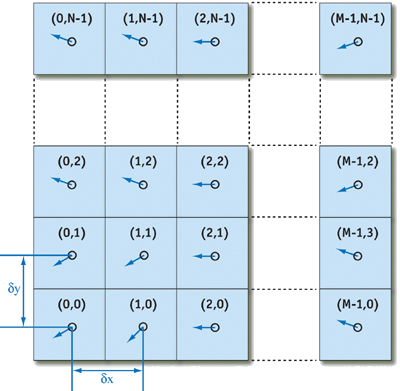
\includegraphics[width=.48\textwidth]{euler.png}
  \caption{Регулярная декартова сетка скоростей.}
\end{figure}

Для численного решения уравнений Навье--Стокса применяется несколько шагов для каждого компонента уравнений в отдельности и обновления значения скоростей в узлах сетки. Одним из самых важных шагов является применение разложения Гельмгольца, которое позволяет объединить градиент давления $\nabla p$ и (\ref{eq:continuity}) в одно уравнение. Другие шаги используют явные, неявные и полуявные методы численного интегрирования. Использование сетки позволяет определять производные, используя метод конечных разностей, основанный на замене производных разностными схемами.

Преимущества метода:
\begin{itemize}
  \item лучшее, по сравнению с другими методами, описание некоторых характеристик жидкости, например поля давлений и плотности.
\end{itemize}

Недостатки метода:
\begin{itemize}
  \item динамичность жидкости ограничена сеткой;
  \item сложности при моделирования смеси жидкостей;
  \item большие затраты памяти для имитации высокого разрешения;
  \item сложность в распараллеливании.
\end{itemize}


\section{Гидродинамика сглаженных частиц Лагранжа}
Гидродинамика сглаженных частиц (ГСЧ) широко используется для моделирования поведения жидкости, газов, астрофизических феноменов и так далее.

ГСЧ является интерполяционным методом для приближения значений и производных непрерывного поля с помощью дискретных точек. Точки определены как сглаженные частицы, которые несут конкретные характеристики, например: массу, положение, плотность, температуру, давление, скорость и др. Характеристики частиц получаются как взвешенные из соседних частиц, то есть влияние каждой частицы на свойства оценивается в соответствии с её плотностью и расстоянием до интересующей частицы. Используемая при этом процедура интерполяции основывается на интегральной аппроксимации функций распределения в виде свёртки так называемым ядром сглаживания с последующей дискретизации вычисления данной свёртки по отдельным частицам.

На каждом шаге вычислительной схемы определяются силы, возникающие в результате вязкости и разности давлений, и внешние силы, после чего определяется ускорение каждой конкретной частицы и, наконец, скорости и координаты.

Преимущества метода:
\begin{itemize}
  \item моделирование в условиях значительной деформации среды, свободными поверхностями и деформируемыми границами;
  \item возможность моделировать смеси жидкостей или газов с разными параметрами;
  \item гарантируется сохранение массы без дополнительных вычислений, так как частицы сами по себе представляют массу;
  \item лёгкость распараллеливания.
\end{itemize}

Недостатки метода:
\begin{itemize}
  \item <<смазывание>> ударных волн и сильных контактных разрывов в большей степени, чем у современных сеточных методов;
  \item необходимо большое количество частиц для создания симуляции с эквивалентной разрешающей способностью сеточным методам.
\end{itemize}
